\capitulo{3}{Conceptos teóricos}

El sistema desarrollado se apoya en la captura, organización, análisis y representación de datos generados durante una sesión de modelado tridimensional. Por ello, este capítulo presenta los conceptos geométricos, temporales y analíticos que justifican las variables registradas y las métricas utilizadas en el proyecto.

El trabajo se sitúa dentro del análisis de la interacción en entornos 3D. En este contexto, cada transformación, cambio de modo, modificación de malla, alteración de vista u operación sobre el modelo puede considerarse una evidencia del comportamiento del usuario. El registro de estos eventos permite estudiar el flujo de trabajo, detectar fases de actividad e inactividad, observar la evolución estructural del modelo y comparar estrategias de creación digital~\cite{jankowski2014,gao2021,gao2023}.

Este capítulo se centra en los fundamentos necesarios para interpretar los datos del sistema: la representación geométrica mediante mallas, la complejidad topológica, las coordenadas UV, las métricas temporales y espaciales, y la relación entre registro, análisis y visualización.

\section{Modelado tridimensional y representación geométrica}

El modelado tridimensional consiste en construir representaciones digitales de objetos situados en un espacio cartesiano definido por tres ejes, normalmente expresados como coordenadas $(X,Y,Z)$. En el modelado poligonal, la estructura principal es la malla, formada por vértices, aristas y caras. La relación entre estos elementos define tanto la forma visible del objeto como su complejidad topológica~\cite{botsch2010polygon}.

\begin{itemize}
    \item \textbf{Vértice}: punto espacial identificado mediante una posición tridimensional. Su número total permite estimar el grado de detalle geométrico del modelo.
    \item \textbf{Arista}: conexión entre dos vértices. Las aristas determinan la continuidad de la estructura y delimitan las caras.
    \item \textbf{Cara}: superficie cerrada por aristas. Puede estar formada por tres vértices, cuatro vértices o más de cuatro vértices.
\end{itemize}

Desde el punto de vista del análisis, la malla no se interpreta solo como una figura visual, sino como una estructura de datos medible. Si durante una sesión aumenta el número de vértices, se puede inferir una fase de construcción o subdivisión. Si aumentan los triángulos o los \textit{n-gons}, puede existir una transformación topológica relevante. Si aparecen variaciones en normales invertidas, el sistema registra posibles problemas de orientación superficial. La Figura~\ref{fig:malla_vertices_aristas_caras} resume visualmente la relación entre vértices, aristas y caras.

\begin{figure}[H]
    \centering
    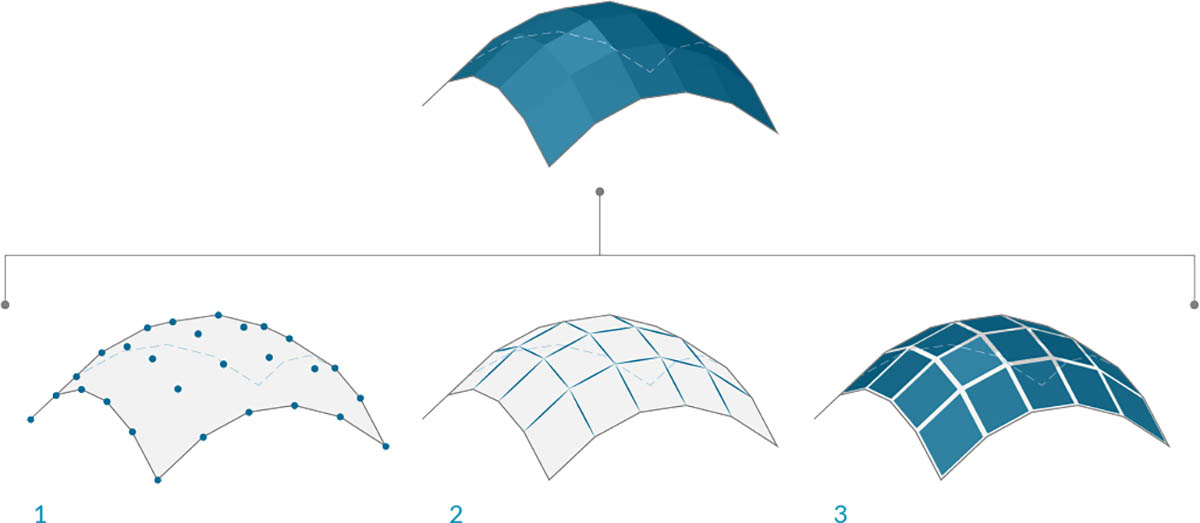
\includegraphics[width=0.85\textwidth]{diagramas/mesh.jpg}
    \caption{Representación conceptual de una malla poligonal mediante vértices 1, aristas 2 y caras 3.}
    \label{fig:malla_vertices_aristas_caras}
\end{figure}

\subsection{Complejidad topológica de la malla}

La topología describe cómo se conectan los elementos de una malla, independientemente de su posición exacta en el espacio. Dos modelos pueden tener una apariencia parecida y, sin embargo, presentar topologías diferentes. Esta diferencia es importante porque la topología condiciona la facilidad de edición, la aplicación de modificadores, la deformación, el sombreado y la preparación técnica del objeto~\cite{botsch2010polygon}.

En este trabajo se consideran tres indicadores especialmente relevantes: variación de vértices, variación de triángulos y variación de \textit{n-gons}. Un aumento de vértices puede indicar subdivisión o incorporación de detalle. Un aumento de triángulos puede reflejar triangulación o cambios derivados de ciertas operaciones geométricas. Un aumento de \textit{n-gons} puede señalar simplificación de superficies o generación de caras complejas. Estas métricas no juzgan de forma aislada la calidad del modelo; proporcionan una señal cuantitativa sobre su evolución.

\subsection{Normales y orientación superficial}

Cada cara de una malla posee una normal, es decir, un vector perpendicular que indica la orientación de la superficie. Las normales se utilizan para calcular iluminación, sombreado y coherencia visual. Cuando una cara está orientada de manera contraria a la esperada, puede producir artefactos de visualización o problemas en etapas posteriores del flujo de trabajo~\cite{botsch2010polygon}.

El sistema registra la variación de normales invertidas mediante la métrica \texttt{NormalDelta}. Una variación positiva puede indicar la aparición de nuevas superficies problemáticas, mientras que una variación negativa puede corresponder a una corrección del modelo. Al integrarse con otras métricas, \texttt{NormalDelta} funciona como un indicador de errores estructurales o de limpieza geométrica.

\section{Espacio UV y correspondencia bidimensional}
\label{subsec:espacio-uv}

Además de la geometría situada en el espacio tridimensional, los modelos pueden disponer de coordenadas UV. El espacio UV es un sistema bidimensional que permite asociar puntos de la superficie del modelo con posiciones en un plano. Esta correspondencia se utiliza para aplicar texturas, organizar islas y preparar la información visual del objeto~\cite{botsch2010polygon}.

El despliegue UV transforma una superficie tridimensional en una representación plana. Durante este proceso, la malla se divide en regiones denominadas islas UV. Cada isla representa una parte de la superficie colocada sobre el plano bidimensional. La relación entre la geometría 3D y el espacio UV es importante porque una edición puede modificar el mapeado de textura sin alterar el número de vértices, caras o aristas del modelo.

Por este motivo, el sistema incorpora la variable \texttt{UV}, que actúa como indicador de trabajo relacionado con coordenadas UV. Esta métrica no mide la calidad absoluta del mapeado, sino la existencia de acciones asociadas al despliegue, empaquetado, reajuste o modificación de coordenadas. En términos analíticos, permite separar las fases dedicadas a la construcción geométrica de las fases dedicadas a la preparación superficial. La Figura~\ref{fig:uv_3d_2d_islas} ilustra esta correspondencia entre la superficie 3D y su despliegue bidimensional.

\begin{figure}[H]
    \centering
    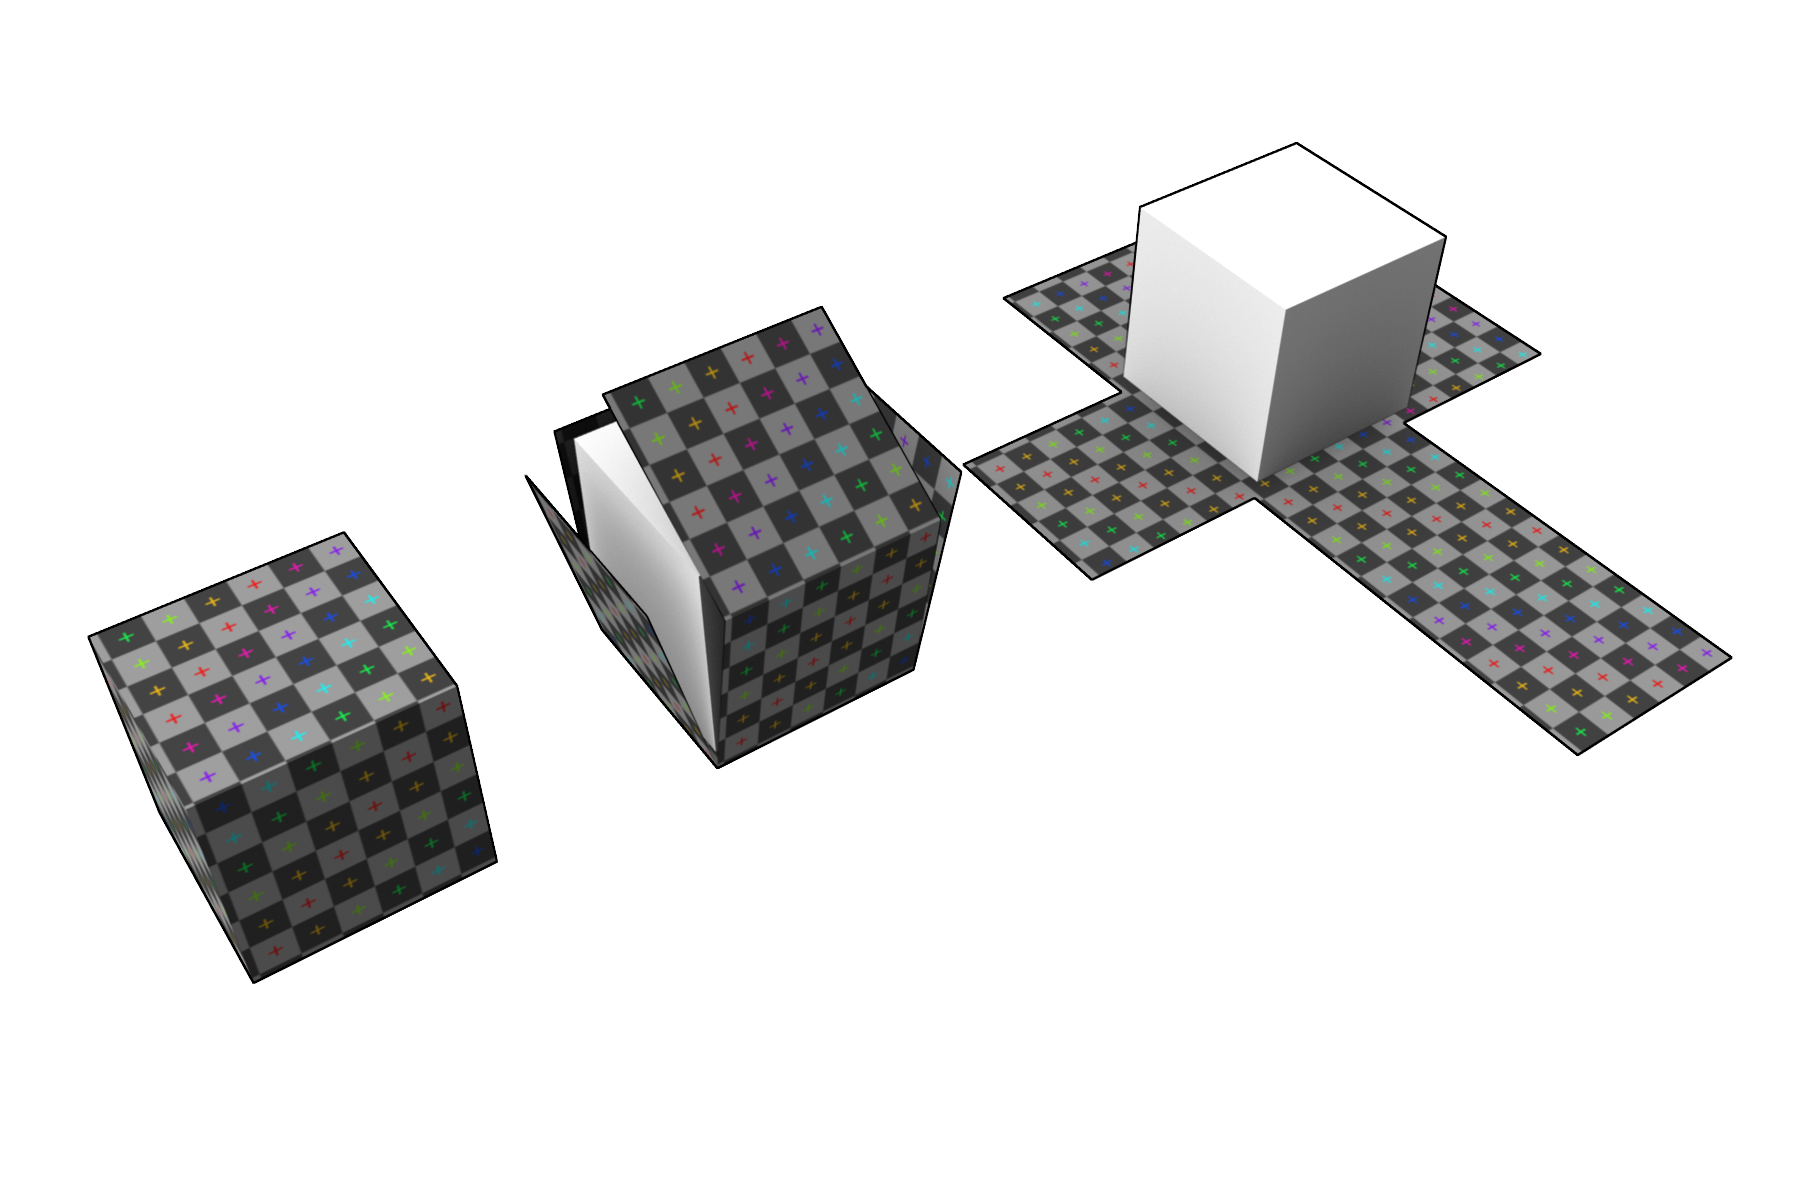
\includegraphics[width=0.9\textwidth]{diagramas/UV.png}
    \caption{Relación conceptual entre una superficie tridimensional y su despliegue en el espacio UV.}
    \label{fig:uv_3d_2d_islas}
\end{figure}

\section{Sistema teórico de métricas del proceso de modelado}

A partir de las variables registradas durante la interacción se define un conjunto de dieciseis métricas analíticas, identificadas como A1--A16. Su objetivo no es valorar únicamente el resultado final del modelo, sino describir el proceso seguido durante su construcción. Esta distinción es importante porque dos modelos visualmente similares pueden generarse mediante estrategias de trabajo muy diferentes: una sesión puede estar basada en duplicaciones y transformaciones rápidas, mientras que otra puede implicar edición manual, cambios topológicos frecuentes o pausas prolongadas~\cite{gao2021,gao2023}.

Las métricas se organizan en cuatro dimensiones principales: temporal, espacial, geométrica y operacional. La dimensión temporal permite estudiar la duración, el ritmo y las pausas de la sesión. La dimensión espacial describe la navegación de la vista y la relación entre el usuario y el objeto activo. La dimensión geométrica resume la evolución de la malla mediante variaciones de vértices, triángulos, \textit{n-gons} y normales. Finalmente, la dimensión operacional recoge acciones que describen la estrategia de construcción, como duplicados, modificaciones, cambios de modo, trabajo UV y cambios en la composición de la escena.

\begin{table}[H]
\centering
\small
\begin{tabularx}{\textwidth}{p{0.10\textwidth}p{0.28\textwidth}X}
\toprule
\textbf{Código} & \textbf{Tipo de métrica} & \textbf{Interpretación teórica} \\
\midrule
A1 & Duración de la sesión & Establece la base temporal del análisis y permite comparar sesiones de distinta longitud. \\
A2--A3 & Pausas e inactividad & Detectan interrupciones o cambios de ritmo dentro del proceso de modelado. \\
A4--A5 & Navegación y proximidad & Describen cómo se desplaza la vista y la distancia relativa respecto al objeto activo. \\
A6--A9 & Picos de movimiento espacial & Identifican instantes de desplazamiento rápido o exploración intensa de la escena. \\
A10 & Reutilización de elementos & Resume acciones como pegado o duplicación, asociadas a estrategias de repetición o aprovechamiento de geometría existente. \\
A11 & Uso de modificadores & Señala fases de ajuste procedural o transformación no destructiva del modelo. \\
A12 & Variación de vértices & Indica incremento, reducción o reorganización de la complejidad geométrica. \\
A13 & Cambios estructurales de malla & Agrupa variaciones en triángulos, \textit{n-gons} y normales invertidas como señal de alteración topológica o corrección geométrica. \\
A14 & Estado de trabajo & Diferencia fases de edición de malla, trabajo en modo objeto u otros estados de interacción. \\
A15 & Actividad UV & Identifica acciones relacionadas con el mapeado bidimensional de la superficie. \\
A16 & Evolución de objetos & Analizan cambios en la composición de la escena mediante creación, eliminación o variación de objetos. \\
\bottomrule
\end{tabularx}
\caption{Interpretación teórica de las métricas A1--A16 empleadas para analizar sesiones de modelado 3D.}
\label{tab:metricas_teoricas_a1_a17}
\end{table}

En conjunto, estas métricas permiten transformar un registro de eventos en una descripción cuantitativa del comportamiento de modelado. No todas representan calidad geométrica de forma directa; algunas describen ritmo de trabajo, otras reflejan navegación espacial y otras resumen operaciones técnicas. Por este motivo, su interpretación debe realizarse de forma conjunta y no como valores aislados~\cite{gao2023}.

\section{Registro temporal de la interacción}

El análisis de una sesión de modelado requiere ordenar los eventos en el tiempo. Para ello, el sistema registra marcas temporales absolutas y valores derivados como minuto y segundo de sesión. A partir de estas columnas se obtiene el tiempo transcurrido y se calculan métricas temporales como duración total, pausas y distribución de pausas por fases~\cite{xie2014}.

La duración total se expresa en minutos mediante la métrica A1. Su valor se calcula como la diferencia entre el primer registro de la sesión y cada registro posterior, dividida entre 3600:

\[
A1_i = \frac{t_i - t_0}{3600}
\]

donde $t_i$ es la marca temporal del registro actual y $t_0$ la marca temporal inicial. Esta métrica establece la base temporal sobre la que se interpretan el resto de indicadores.

Las pausas se estiman mediante la métrica A2. Una pausa se identifica cuando el intervalo entre dos registros consecutivos es anormalmente alto en relación con la media y la desviación típica de los intervalos positivos:

\[
\theta_p = \overline{\Delta t} + 2\sigma_{\Delta t}
\]

Si $\Delta t_i \geq \theta_p$ y no se detecta evento de edición asociado, el intervalo se interpreta como pausa. La métrica A3 reutiliza esta detección para estudiar la distribución de pausas por fases temporales, normalmente dividiendo la sesión en cuartiles.

\section{Métricas espaciales de navegación y proximidad}

Durante una sesión, el usuario modifica la posición de la vista para inspeccionar el modelo desde diferentes perspectivas. Esta navegación espacial se registra mediante las coordenadas \texttt{UserX}, \texttt{UserY} y \texttt{UserZ}. Aunque estas coordenadas no describen cambios directos en la geometría, sí aportan información sobre cómo se explora el objeto~\cite{jankowski2014,lavioila2017}.

La velocidad de movimiento de la vista se calcula mediante la distancia euclídea entre dos posiciones consecutivas dividida por el tiempo transcurrido:

\[
v_i = \frac{\lVert P_i - P_{i-1} \rVert}{t_i - t_{i-1}}
\]

donde $P_i=(x_i,y_i,z_i)$ representa la posición de la vista en el instante $i$. La métrica A4 expresa esta velocidad en unidades por hora para facilitar su comparación a lo largo de la sesión.

La proximidad al objeto se calcula con la métrica A5. Para ello se compara la posición de la vista con el centro del objeto activo y se descuenta el radio aproximado del objeto:

\[
d_i = \max(\lVert P_i - O_i \rVert - r_i, 0)
\]

donde $O_i$ es el centro del objeto y $r_i$ su radio. Un valor bajo indica inspección cercana, mientras que un valor alto sugiere una vista general de la escena.

Las métricas A6, A7, A8 y A9 se basan en picos de velocidad espacial. Para identificarlos, se calcula un umbral de velocidad:

\[
\theta_v = \overline{v}_{+} + 2\sigma_{v_{+}}
\]

Los instantes cuya velocidad supera este umbral se interpretan como manipulaciones rápidas de vista o desplazamientos espaciales destacados.

\section{Métricas de estrategia y evolución del modelo}

Las métricas estratégicas describen acciones que no se explican únicamente por la geometría resultante, sino por la forma en la que el usuario avanza durante la construcción del modelo. En este grupo se incluyen duplicados, pegado, uso de modificadores, variaciones de malla, cambios de modo, trabajo UV y cambios de objeto~\cite{gao2021,liu2022}.

La métrica A10 agrupa acciones de aceleración basadas en \texttt{CtrlV}, \texttt{ShiftD} y \texttt{AltD}:

\[
A10_i = |CtrlV_i| + |ShiftD_i| + |AltD_i|
\]

Esta métrica permite identificar estrategias de reutilización de elementos. Un valor elevado puede indicar construcción por duplicación, repetición de componentes o aprovechamiento de geometría existente.

La métrica A11 mide variaciones en modificadores mediante \texttt{ModifierDelta}. Registra fases de ajuste técnico o exploración procedural. La métrica A12 representa la evolución de vértices mediante \texttt{VertexDelta}; un valor positivo indica incremento de complejidad geométrica y un valor negativo puede señalar simplificación, eliminación o fusión.

La métrica A13 agrupa errores o cambios estructurales de malla mediante la suma absoluta de \texttt{NgonDelta}, \texttt{TriDelta} y \texttt{NormalDelta}:

\[
A13_i = |NgonDelta_i| + |TriDelta_i| + |NormalDelta_i|
\]

El uso del valor absoluto permite medir la intensidad del cambio sin diferenciar si el valor aumenta o disminuye. Por ejemplo, en una sesión de modelado puede ser relevante saber que ha cambiado el número de triángulos, \textit{n-gons} o normales invertidas, aunque el cambio corresponda a una creación, eliminación o corrección de geometría.

La métrica A14 identifica el estado de trabajo del usuario. Se asigna un valor distinto según el modo activo: edición de malla, modo objeto u otros estados. Esta codificación permite distinguir si la actividad registrada corresponde a una fase de edición directa de la geometría o a una fase de manipulación general de objetos.

La métrica A15 registra la existencia de actividad relacionada con coordenadas UV. Su finalidad es detectar momentos en los que el usuario trabaja sobre el mapeado bidimensional de la superficie, aunque la geometría principal de la malla no cambie.

Por último, la métrica A16 describe cambios en la composición de la escena, por lo que permite saber si se han añadido o eliminado objetos. 

\section{Formato CSV y estructura tabular de los datos}

El formato CSV (\textit{Comma-Separated Values}) permite almacenar información en forma de tabla, donde cada fila representa una observación y cada columna describe una variable. En el contexto de una sesión de modelado tridimensional, esta estructura resulta adecuada porque permite ordenar cronológicamente los eventos registrados y relacionarlos con variables temporales, espaciales, geométricas y operacionales~\cite{mckinney2022python}.

Desde un punto de vista teórico, el CSV actúa como una representación intermedia entre la interacción del usuario y el cálculo posterior de métricas. Las acciones realizadas durante el modelado no se analizan directamente como eventos aislados, sino como una secuencia estructurada de registros. Esta organización permite transformar la actividad observada en series temporales comparables, resúmenes estadísticos y visualizaciones~\cite{vanderalst2016process}.

La estructura tabular también facilita la separación entre captura y análisis. El módulo de registro puede limitarse a almacenar los cambios relevantes de la sesión, mientras que el módulo de análisis interpreta posteriormente esos datos y calcula los indicadores correspondientes. De este modo, el CSV funciona como un puente entre el proceso de modelado y la explotación analítica de la información.

\section{Visualización analítica en tres dimensiones}

La visualización de datos permite interpretar resultados que serían difíciles de comprender mediante tablas aisladas. En este proyecto, las métricas calculadas pueden representarse como trayectorias, puntos, radares o gráficas temporales. La elección de la representación depende del tipo de variable: las métricas temporales se interpretan mejor como evolución, las espaciales como recorrido o proximidad, y las estratégicas como frecuencia o intensidad de acción~\cite{munzner2014visualization}.

La representación tridimensional aporta una ventaja conceptual cuando los datos proceden de una tarea espacial. Por ejemplo, la trayectoria de la vista puede relacionarse con la posición del objeto; los picos de velocidad pueden localizarse en momentos específicos de la sesión; y la evolución de vértices o errores puede compararse con fases de navegación intensa.

\section{Relación conceptual entre registro, métricas y visualización}

La información del sistema sigue un recorrido progresivo desde la acción del usuario hasta la interpretación final de los resultados. Primero, el usuario realiza acciones durante el modelado, como mover la vista, transformar un objeto, modificar una malla, cambiar coordenadas UV o añadir y eliminar elementos de la escena. Después, el sistema registra esas acciones en un archivo CSV mediante columnas específicas. Finalmente, el módulo de análisis utiliza esos datos para calcular métricas y generar visualizaciones.

De esta forma, el CSV no se utiliza únicamente como un archivo de almacenamiento, sino como una estructura intermedia entre la sesión de modelado y el análisis posterior. Cada columna registrada aporta información concreta: unas columnas permiten ordenar los eventos en el tiempo, otras describen posiciones y distancias, otras recogen cambios geométricos y otras identifican operaciones realizadas por el usuario.

Esta organización permite justificar por qué se registran esas variables y no otras. El objetivo no es describir solamente una herramienta, sino mostrar cómo los datos temporales, espaciales, geométricos y operacionales pueden utilizarse para analizar el proceso de modelado tridimensional~\cite{gao2021,gao2023}.